%%%%%%%%%%%%%%%%%%%%%%% file template.tex %%%%%%%%%%%%%%%%%%%%%%%%%
%
% This is a template file for Web of Conferences Journal
%
% Copy it to a new file with a new name and use it as the basis
% for your article
%
%%%%%%%%%%%%%%%%%%%%%%%%%% EDP Science %%%%%%%%%%%%%%%%%%%%%%%%%%%%
%
%%%\documentclass[option]{webofc}
%%% "twocolumn" for typesetting an article in two columns format (default one column)
%
\documentclass{webofc}
\usepackage[varg]{txfonts}   % Web of Conferences font
%
% Put here some packages required or/and some personnal commands
\usepackage{url}
% \usepackage{cite}
\usepackage{lineno}
\linenumbers
%
\begin{document}
%
\title{Experiences and developments of the RAL-LCG2 Tier-1object store ECHO in Run-3 and preparing for HL-LHC}
%
% subtitle is optionnal
%
%%%\subtitle{Do you have a subtitle?\\ If so, write it here}

\author{\firstname{J} \lastname{Walder}\inst{1}\fnsep\thanks{\email{james.walder@stfc.ac.uk}} \and
\firstname{T} \lastname{Byrne}\inst{1}\and
\firstname{A} \lastname{Dewhurst}\inst{1}  \and
\firstname{I} \lastname{Johnson}\inst{1}  \and
\firstname{A} \lastname{Rogovskiy}\inst{1}  \and
\firstname{J} \lastname{Thomas}\inst{1}
}

\institute{STFC Rutherford Appleton Lab, Harwell, UK}

\abstract{%
Data storage at the UK Tier-1 facility at RAL is provided through its ECHO storage, serving the requirements for the WLGC and increasing numbers of other HEP and astronomy related communities.
ECHO is a Ceph-backed erasure-coded object store, currently providing in excess of 40PB of usable space, with frontend access to data provided via XRootD or gridFTP, using the libradosstriper library of Ceph. 
The storage must service the needs of: high-throughput compute, with staged and direct file access passing through an XCache on each workernode; data access to compute running at storageless satellite sites; and, managed inter-site data transfers using the recently adopted HTTPS protocol (via WebDav), which includes multi-hop data transfers to and from RAL's newly commissioned CTA tape endpoint.
A review of the experiences of providing data access via an object store within these data workflows is presented, including the details of the improvements necessary for the transition to WebDav, used for most inter-site data movements, and enhancements for direct-IO file access, where the development and optimisation of buffering and vector read strategies is explored.}
%
\maketitle
%
\section{Introduction\label{intro}}
The Rutherford Appleton Laboratory (RAL) plays a crucial role in supporting the data-intensive requirements of the Worldwide LHC Computing Grid (WLCG). To facilitate efficient data access and storage for high-energy physics experiments, RAL has established the ECHO~\cite{dewhurst2017deployment,echoChep20} infrastructure. This infrastructure combines the XRootD~\cite{xrootd} and Ceph~\cite{ceph} technologies to provide a robust and scalable solution for handling vast amounts of data.

One of the primary use cases is the distribution of experimental data generated at various Large Hadron Collider (LHC) experiments, i.e. ALICE, ATLAS, CMS and LHCb. The ECHO cluster employs XRootD as a high-performance data interface allowing researchers worldwide to efficiently retrieve and replicate these datasets for analysis.
To enhance data redundancy and reliability, the ECHO infrastructure leverages Ceph's distributed storage capabilities. This redundancy ensures that data remains accessible, even in the face of hardware failures or other unforeseen issues. 

In preparation for Run-3 of the LHC, and to prepare for the requirements of HL-LHC, a number of optimisations and updates have occured since the original deployement of ECHO, such as the migration~\cite{Bockelman_2020} from gridFTP~\cite{allcock2001gridftp} to WebDav~\cite{webdav}. 
A review of the changes to ECHO to meet these challenges that have been adapted so far, focusing on XRootD, is provided in this note. 

\section{ECHO and the Ceph storage cluster\label{ceph}}
ECHO is built on the Ceph distributed storage platform, which offers unified and scalable storage capabilities. Ceph uses a distributed architecture consisting of storage nodes, known as Object Storage Devices (OSDs), to store data. These OSDs are distributed across the cluster for load balancing and redundancy. 

To optimise storage efficiency, ECHO employs erasure coding (EC) techniques. This method reduces data replication overhead while maintaining data integrity and availability. Erasure coding is particularly useful for large-scale, exabyte-sized storage systems like ECHO. For the data pools currently used by the major experiments, $8+3$ EC is used. 

At the time of writing, approximately $80$~PB of raw storage is deployed for use, with over 6000 OSDs across approximately 300 Storage Nodes (SN). 
A host level failure domain is used, such that the distribution of data in placement groups across the OSD means that failure of any single SN will not risk the integrity of the data. 

\subsection{Data storage\label{datastore}}
While RAL and its ceph storage provides for CephFS, S3 and SWIFT endpoints, the data stored for the experiments uses the ceph as an Object Store, interacting at the rados layer using functionality provided by the libradosstriper~\cite{libradosstriper} and {\em XrdCeph}~\cite{libradosstriper} plugin to XRootD (described below). 
In practice, with the implementation of ECHO, this means that a file writen to echo is divided into $64$~MiB ceph objects, with name suffixed with a 16-digit 0-padded hex number (incrementing by one for each object) before being written into Ceph, and with the EC applied. Figure~\ref{fig_striper} illustrates the way a typcial file would be stored on ECHO. In Fig.~\ref{fig_osddist}, the distribution of data across OSDs and SNs is shown. In this example, the file is divided into 157~ceph objects, which are placed over 1400~OSDs on approximately 230~SNs. i.e. data occupies approximately 6 OSDs per SN and a large (say 10~GiB) is likely to be distributed across most SNs of the ceph cluster. 
%
\begin{figure}[h]
\centering
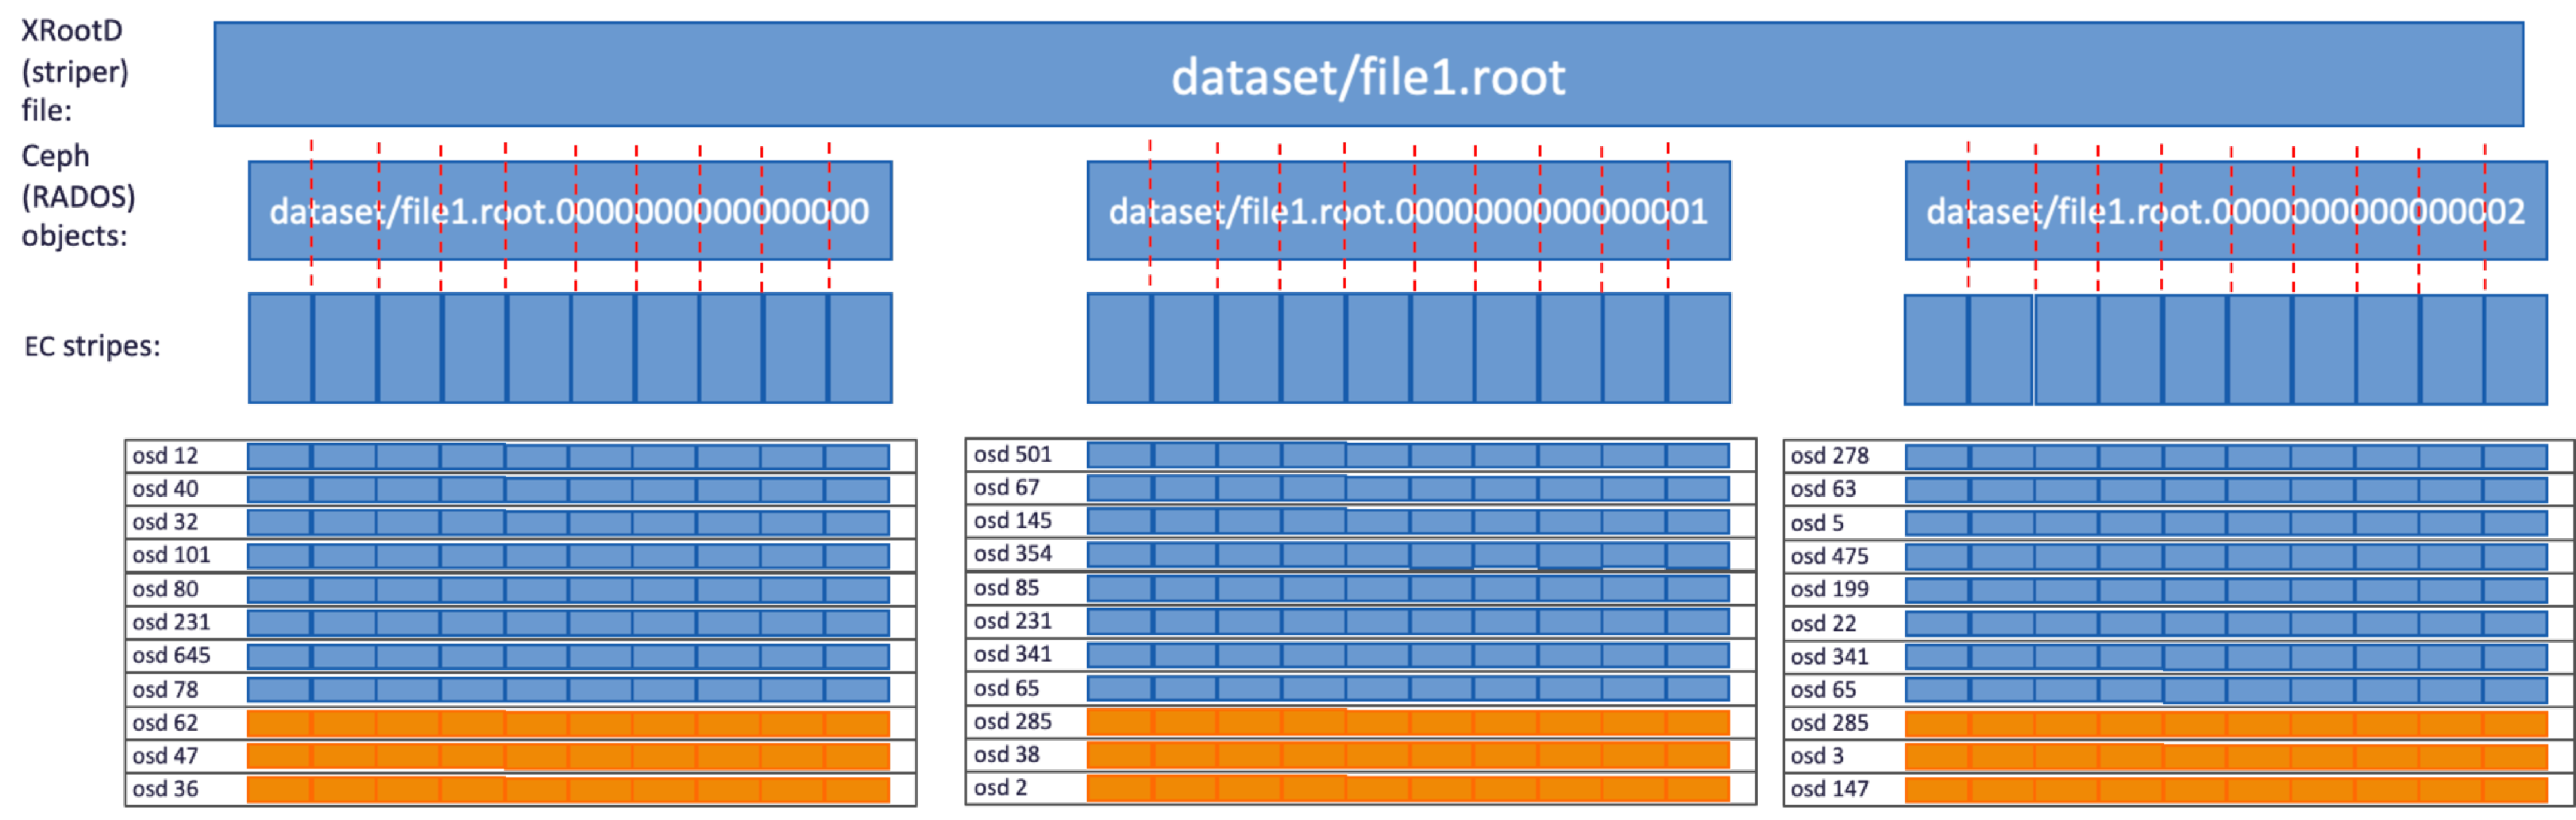
\includegraphics[width=\textwidth,clip]{figures/radosstriper.pdf}
\caption{For a typical file on ECHO, the libradosstriper divides the file into (a configurable) $64$~MiB objects, with each object then being striped and erasure coded across the OSDs of the placement groups.}
\label{fig_striper}       % Give a unique label
\end{figure}
%
\begin{figure}[h]
     \centering
     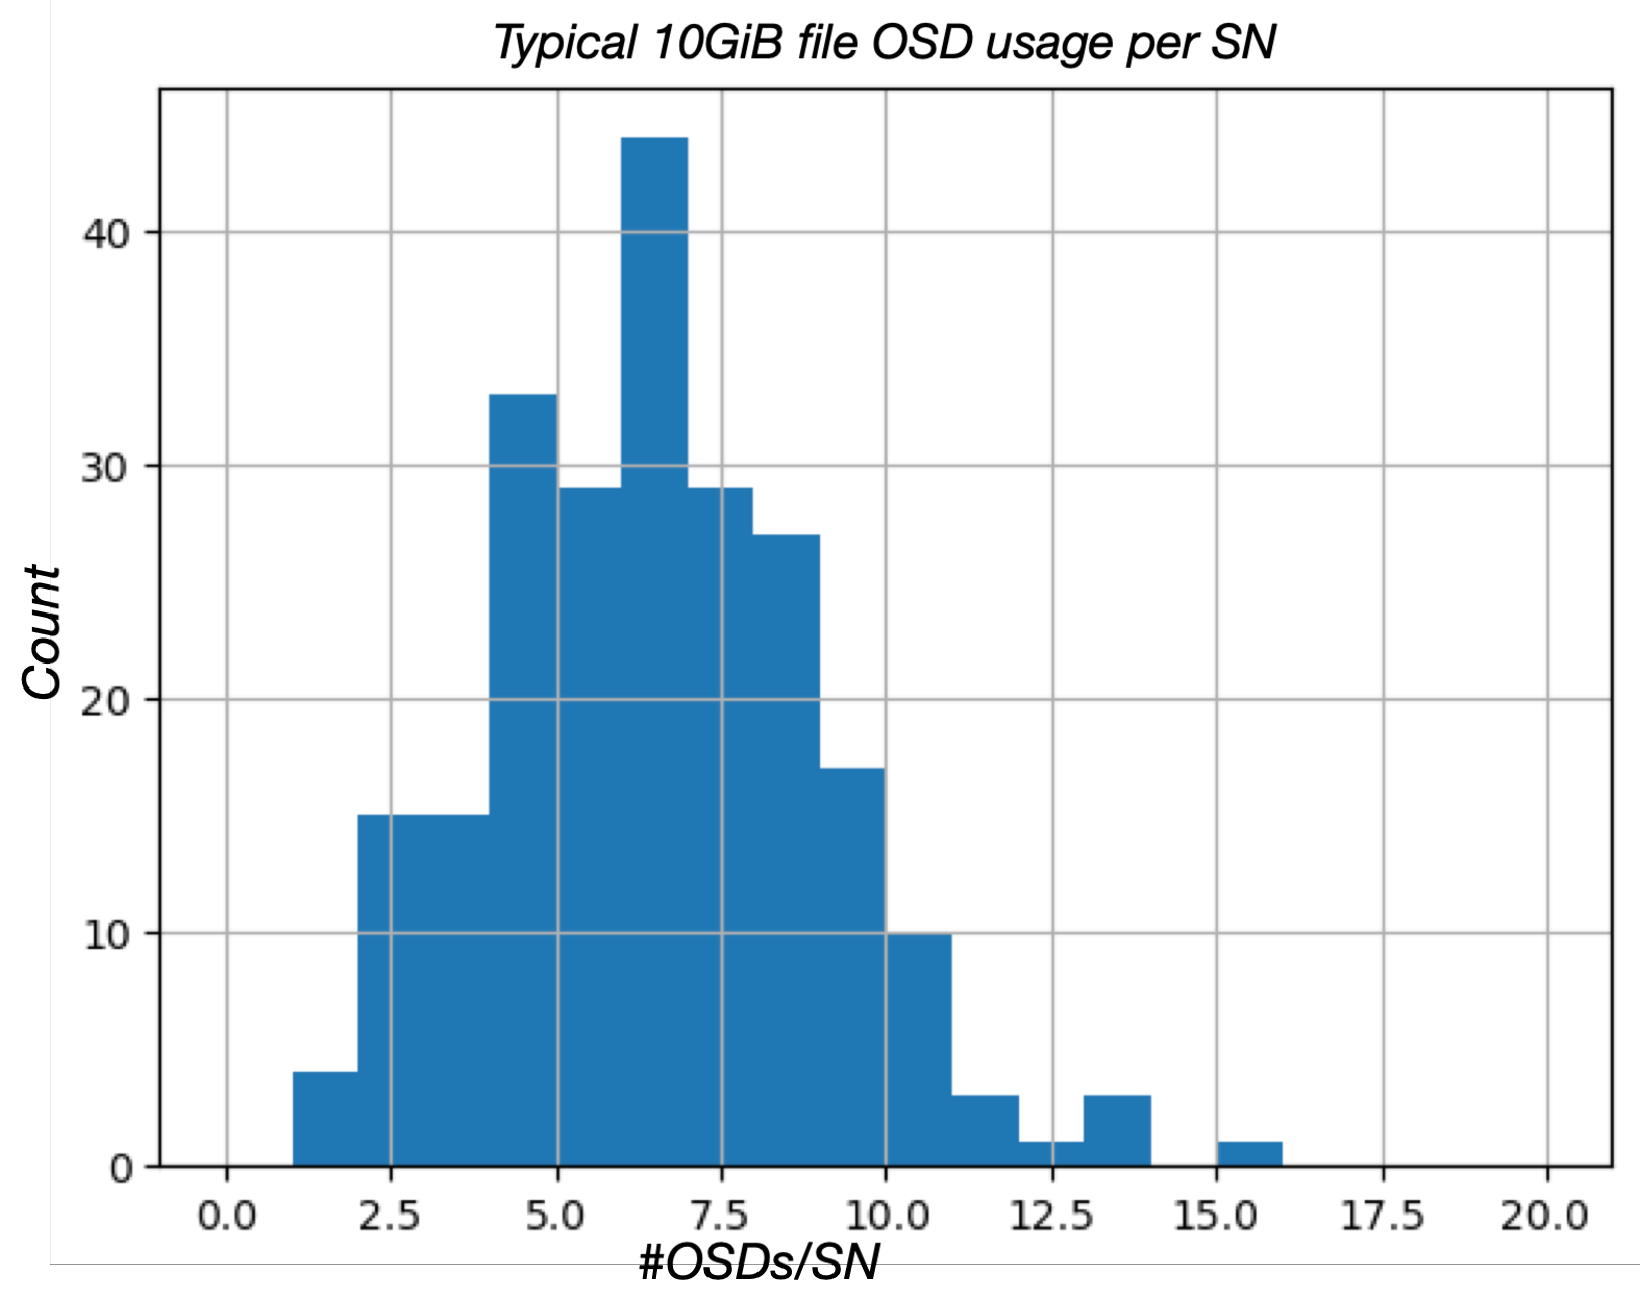
\includegraphics[width=5cm,clip]{figures/osds.pdf}
     \caption{For a 10~GiB file, a typical distribution of the number of OSDs that data is distibuted across per storage node.}
     \label{fig_osddist}       % Give a unique label
\end{figure}



\section{XRootD and data access\label{sec:xrd}}
While Ceph provides the storage backend, an interface is required for clients to interact with it. XRootD~\cite{xrootd} provides a lightweight and flexible framework that satifies the needs for WLCG and other communities. In addition, its plugin style design allowed for the development of the XrdCeph plugin~\cite{libradosstriper} to bridge between XRootD and the rados layer of Ceph. 
XrdCeph inherites from the {\em XrdOss} layer to provide this interface and to also present a restricted set of access operations. For example, as an object has no concept of directory hierarchy, and as a listing over all object in a (large) ceph pool is prohibitly expensive, no possibly to list files is available. Similarly, as a rename operation is effectivly a copy to a new name, with resultant movement of data across to new OSDs and placement groups, this is also a non implemented feature. 
XrdCeph uses the libradosstriper library of Ceph. This provides for mostly atomicaly correct behaviour, however, and as will be discussed below, due it locking and unlocking behaviour is not always optimal for small reads. In the case of high-energy physics, the majority of use-cases are Write Once, Read Many (WORM) requests. 

% \subsection{XRootD architecture for ECHO\label{xrootdsetup}}


\section{Improving performance for Run-3 and beyond\label{sec:requirements}}
With the evolution to run-3 and improvements and changes in other layers of the middleware, ECHO (including XrdCeph) has needed adapt to these changes. 
These changes include the deprication of GridFTP, in favour of WebDAV, resulting in signficant usage of XrdCeph compared to the GridFTP implementation~\cite{gridftpplugin,dewhurst2017deployment}. The use of paged reads and wrties in xroot protocol transfers, which effectively moves reads and writes to small ($<100kb$) reads and writes from (typcially) 8~MiB blocks. Here, and with the design of libradosstriper and XrdCeph, small reads and writes were not efficient against Ceph, due to its locking and unlocking behaviour. 

With the initial design of XrdCeph vector reads\footnote{Vector reads are typically used in direct access from jobs running on worker nodes to access directly only the bytes of data that are useful for the client, rather than downloading the entire file.} are not supported in XrdCeph, which means that for requests of sparse reads, these reads were unfolded into a set of small read requests, and hence suffered from significant overheads.

To overcome these challenges and to continue to improve the throughput for Echo, two strategies were deployed. Firstly an attempt to place a simple buffering layer in XrdCeph was deployed. For Reads, when a read was requested, if the data was already not in the buffer, a request to ceph is issued for a single read, the size of the buffer, thus preventing small reads from being directly made against libradosstriper and Ceph. Similarly, for writes, once the buffer was full, a single write is made to Ceph via libradosstriper, ensuring that small writes are not propagated through. 
Secondly, for reads, it should be possible to bypass the locking and unlocking behaviour in XrdCeph, where significant overhead on small reads can be introduced, and additionally implementing efficient vector read support at the librados layer~\cite{tomceph23} (rather than in libradosstriper).

\subsection{Buffering in XrdCeph\label{buffer}}
The performance of introducing a buffer into the XrdCeph layer is showin in Fig.~\ref{fig:buffering}.
For davs, reads and writes are typically requested (within the XRootD framework) in 1~MiB blocks. For root protocol transfers, these requests can range from approximately $64kb$ for paged requests to 8~MiB. The plots show the performance for single file transfers in a development cluster environment. In production, a buffer size of 16~MiB was empirically found to optimise throughput and memory usage. This approach is fully efficient (in terms of data read from Ceph) for cases where the whole file is read. In cases where on small and sparse sections of the file is read, this appoach can lead to inefficiencies in reading uncessary data. 
With this buffering, no attempt was made to buffer explicit vector read requests for this reason. 
%
\begin{figure}[h]
     \centering
     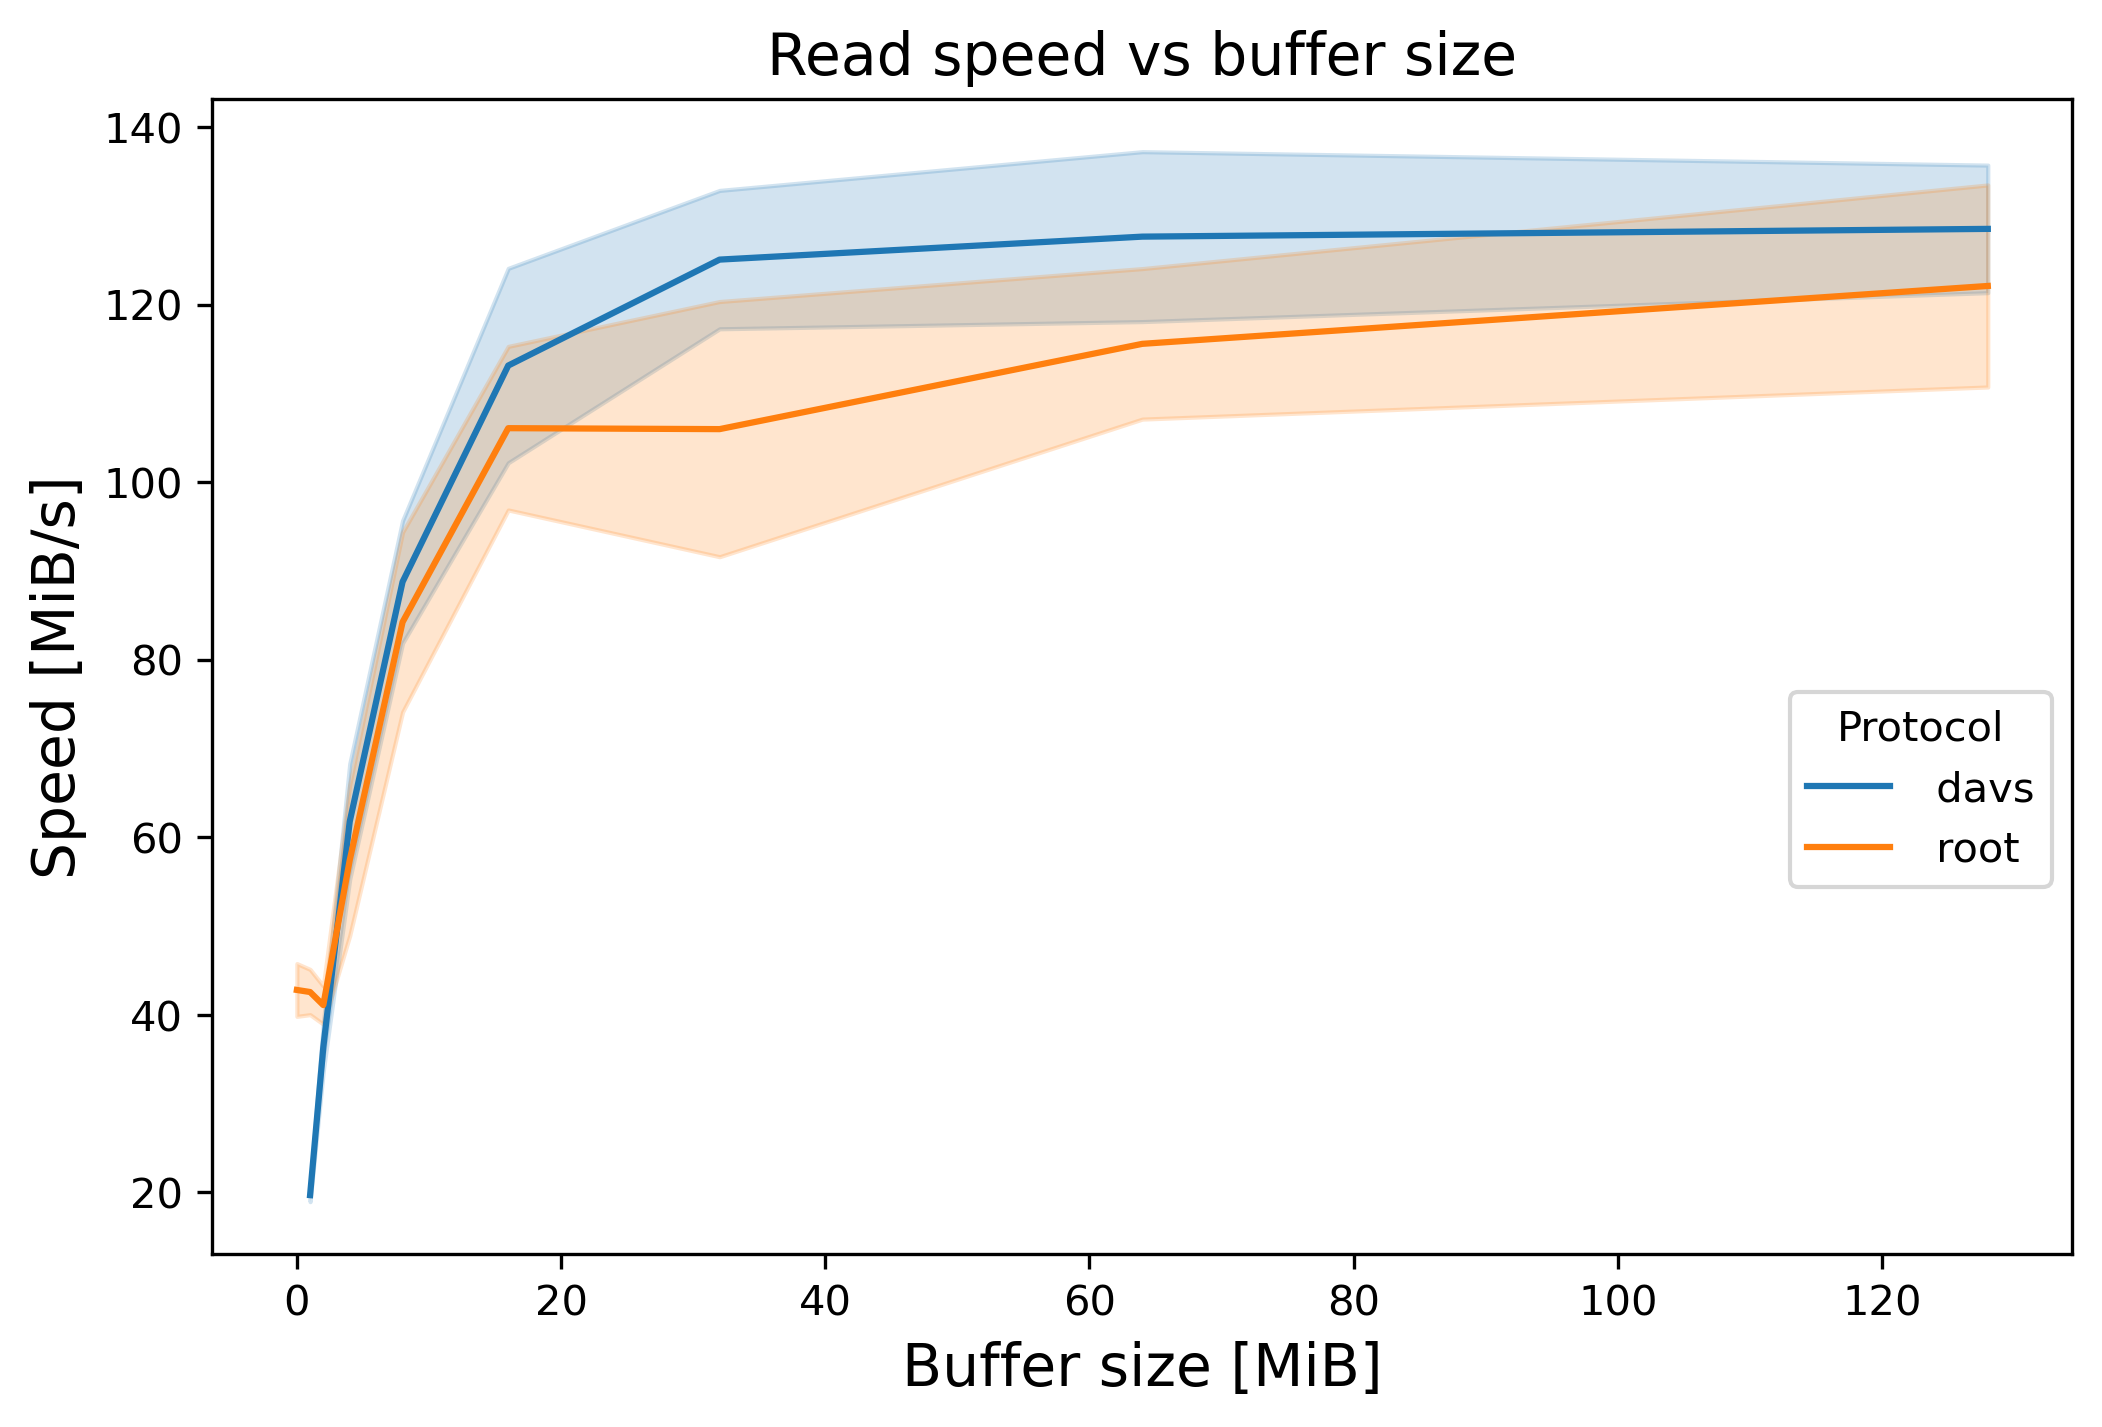
\includegraphics[width=0.45\textwidth,clip]{figures/fig_read_speed.png}\hfil
     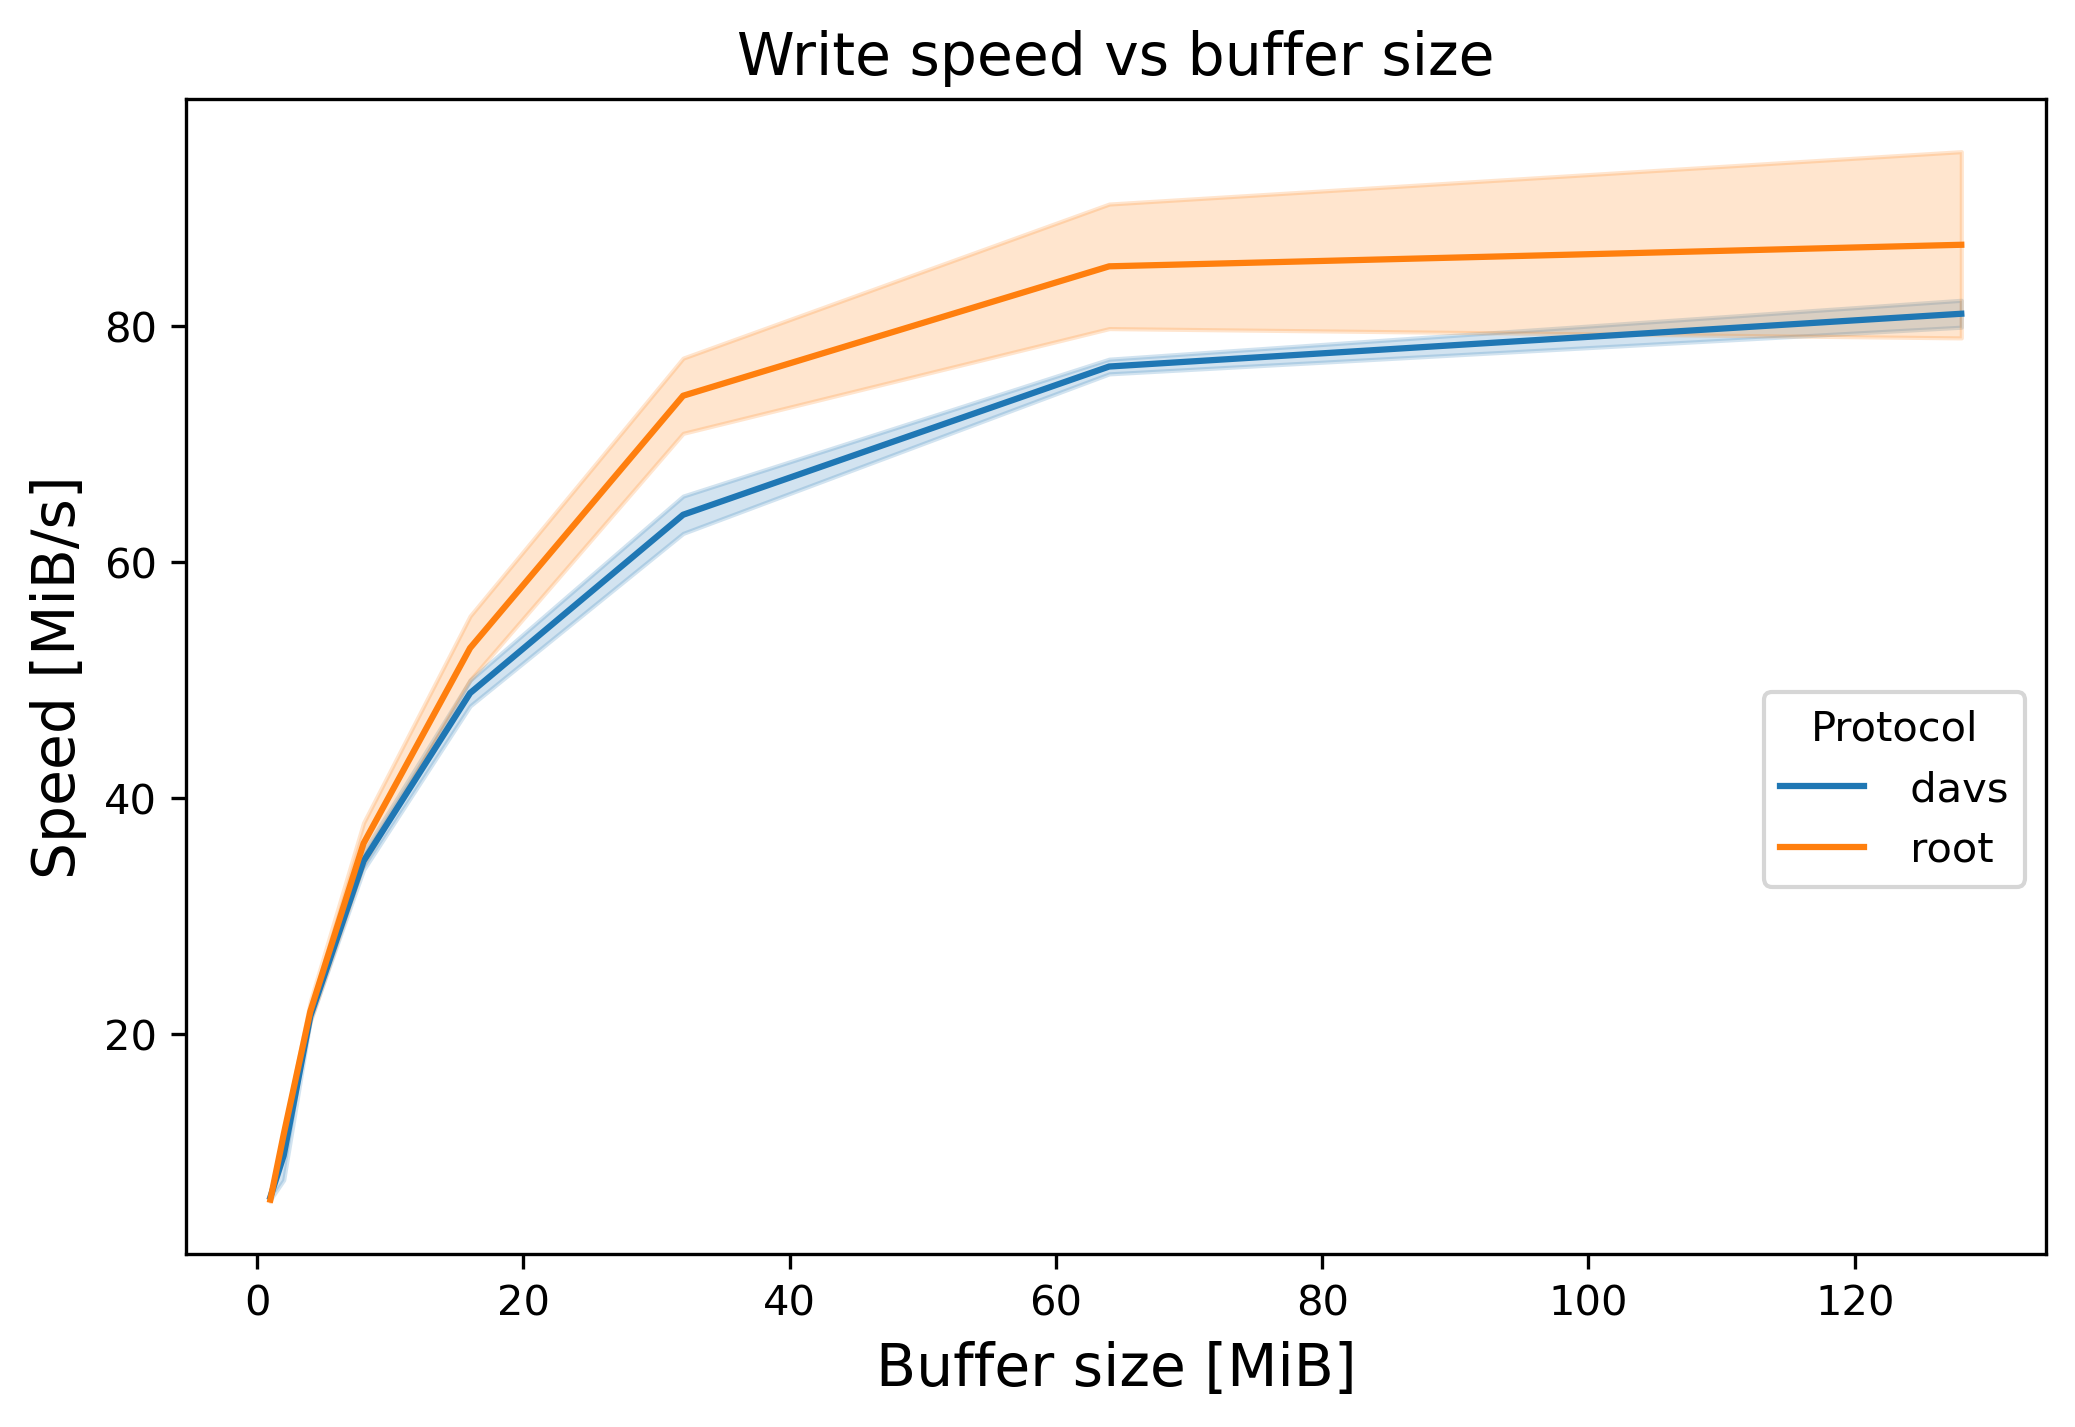
\includegraphics[width=0.45\textwidth,clip]{figures/fig_write_speed.png}
     \caption{Performance of read~(left) and write~(right) speed for different sizes of XrdCeph buffer, measured using root and davs protocols for a 1~GiB file. The lines represent the mean of the distribution for each buffer size, and the colour bands indicate the statistical uncertainty.}
     \label{fig:buffering}       % Give a unique label
\end{figure}

\subsection{Striperless reads and read vector implementation\label{sec:striperless}}
The second strategy employed to improve throughput for reads and vector reads (write requests are not touched by these changes) was to remove libradosstriper -- removing the locking and unlocking steps -- and to implement efficient vector read support. 
Technicaly, some aspects of libradosstriper are reimplemented, such as the functionality to map between a read's offset and size onto the local offset and read lenght of each ceph object, noting that a read could cover multiple objects. The removal of locking for reads has very limited practical concerns, given the WORM nature of operations.

In Fig.~\ref{fig:bufferingnostriper} the read data taken from Fig.~\ref{fig:buffering} is shown, together with data taken using the non-striper reads, for differing sizes of buffer. While the data suggests that the non-striper implementation is most performant with no -- or very small -- buffer sizes, when tested in the production environment, the large number of small reads could still have a negative impact on the performance of the buffer, hence it is still useful to keep some degree of buffering. 
%
\begin{figure}[h]
     \centering
     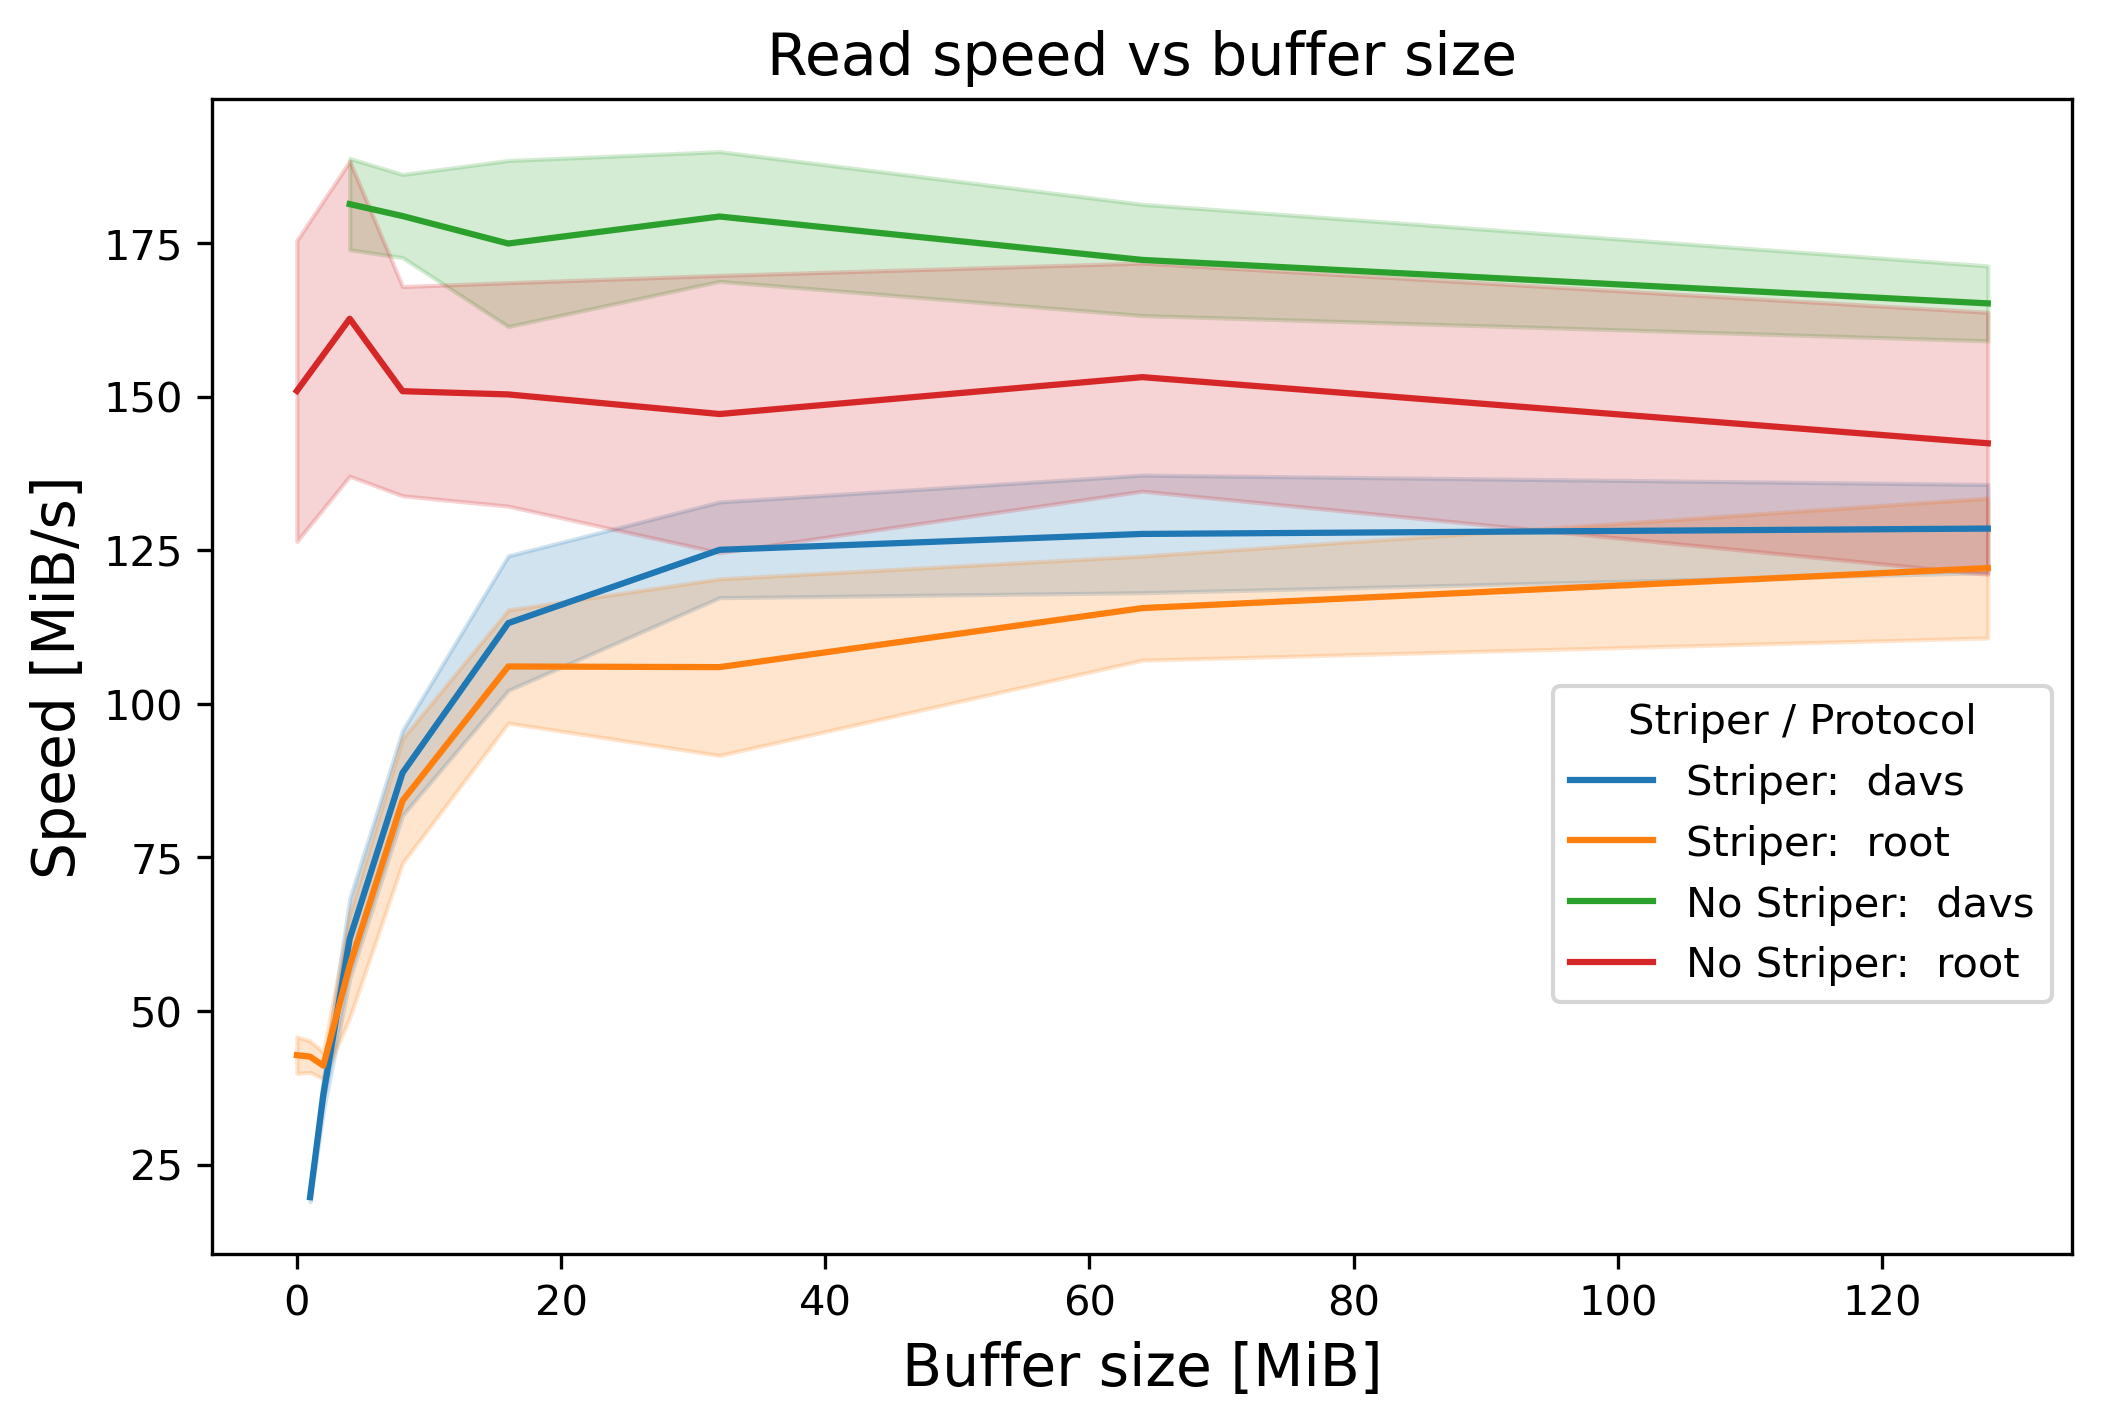
\includegraphics[width=0.45\textwidth,clip]{figures/fig_read_speed_comined.png}\hfil
     \caption{Performance of read speeds for different sizes of XrdCeph buffer, measured using root and davs protocols for a 1~GiB file. In addition to the curves overlaid from Fig.~\ref{fig:buffering}, the effect of reads without the libradosstriper are shown, also for various sizes of buffer.}
     \label{fig:bufferingnostriper}       % Give a unique label
\end{figure}



For the vector reads, the set of reads (described by a list of offsets and read-lengths) are mapped to their ceph objects, and a local set of offset and lengths. These sets are then issued to ceph via librados in a batched operation. This replaces the default operation that converts each chunk of the vector read into a single read, into a small set of batched read requests.
Figure~\ref{fig:readv} compares the performance between the default implementation and the updated reads. The test procedure is as follows: 
\begin{itemize}
     \item For each test 32 processes are submitted simultaneously;
     \item Each process connects to the storage, executes 100 readv requests, then disconnects; the procedure is repeated 10 times (i.e. each process submits 1000 readvs overall);
     \item Each individual readv request has 900 chunks;
     \item Chunks are distributed over 42 MiB;
     \item The length of every chunk is distributed between 1 and 1024 bytes.
\end{itemize}
The improvements are visible through both the lack of failed reads, and improvements in the mean and meadian read times from $6.0$~s to $1.1$~s and from $0.84$~s to $0.73$~s, respectively. 
%
\begin{figure}[h]
     \centering
     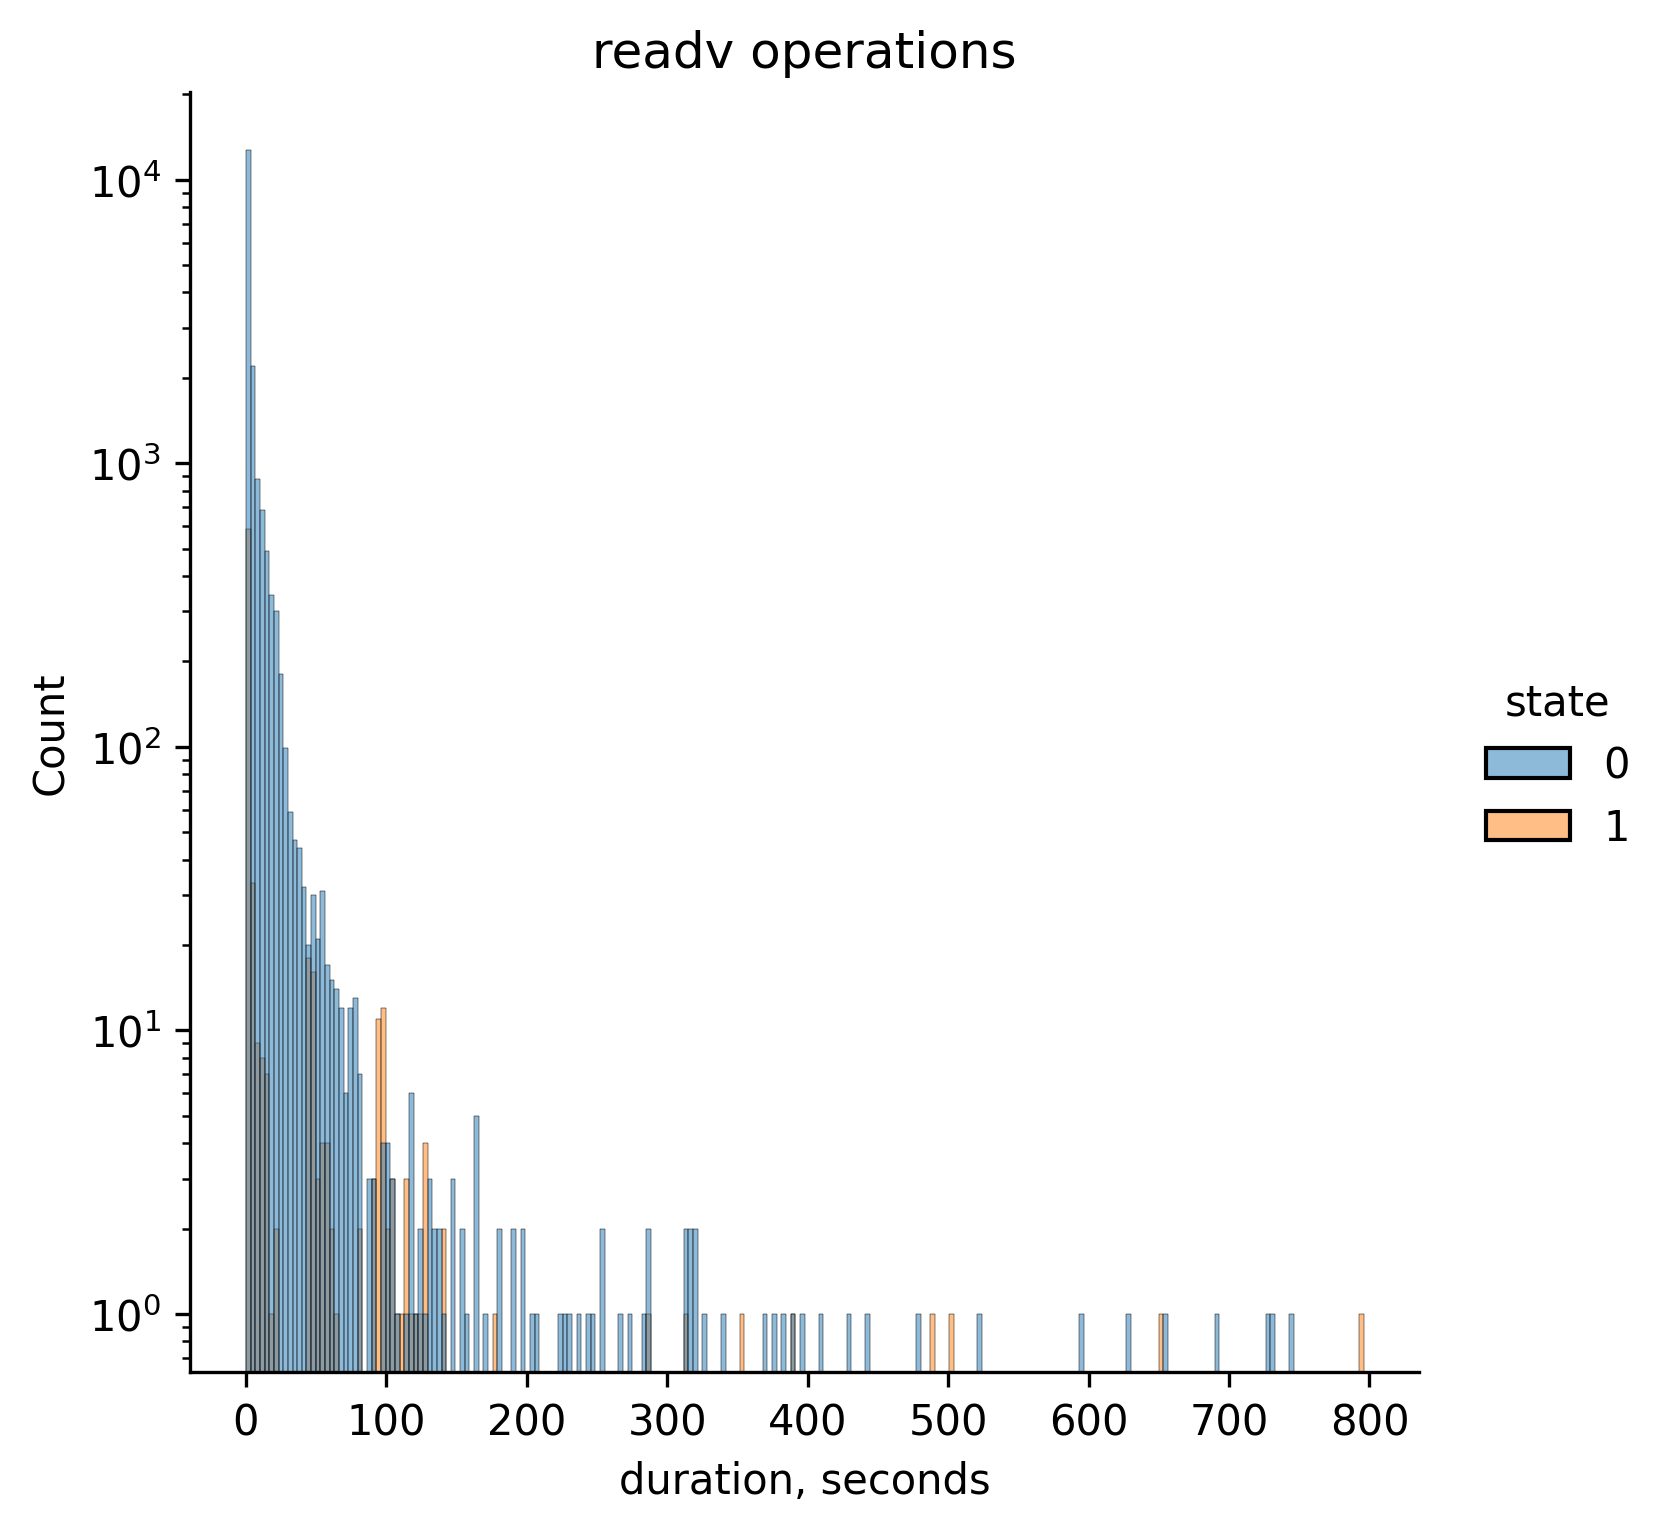
\includegraphics[width=0.45\textwidth,clip]{figures/readv_original.png}\hfil
     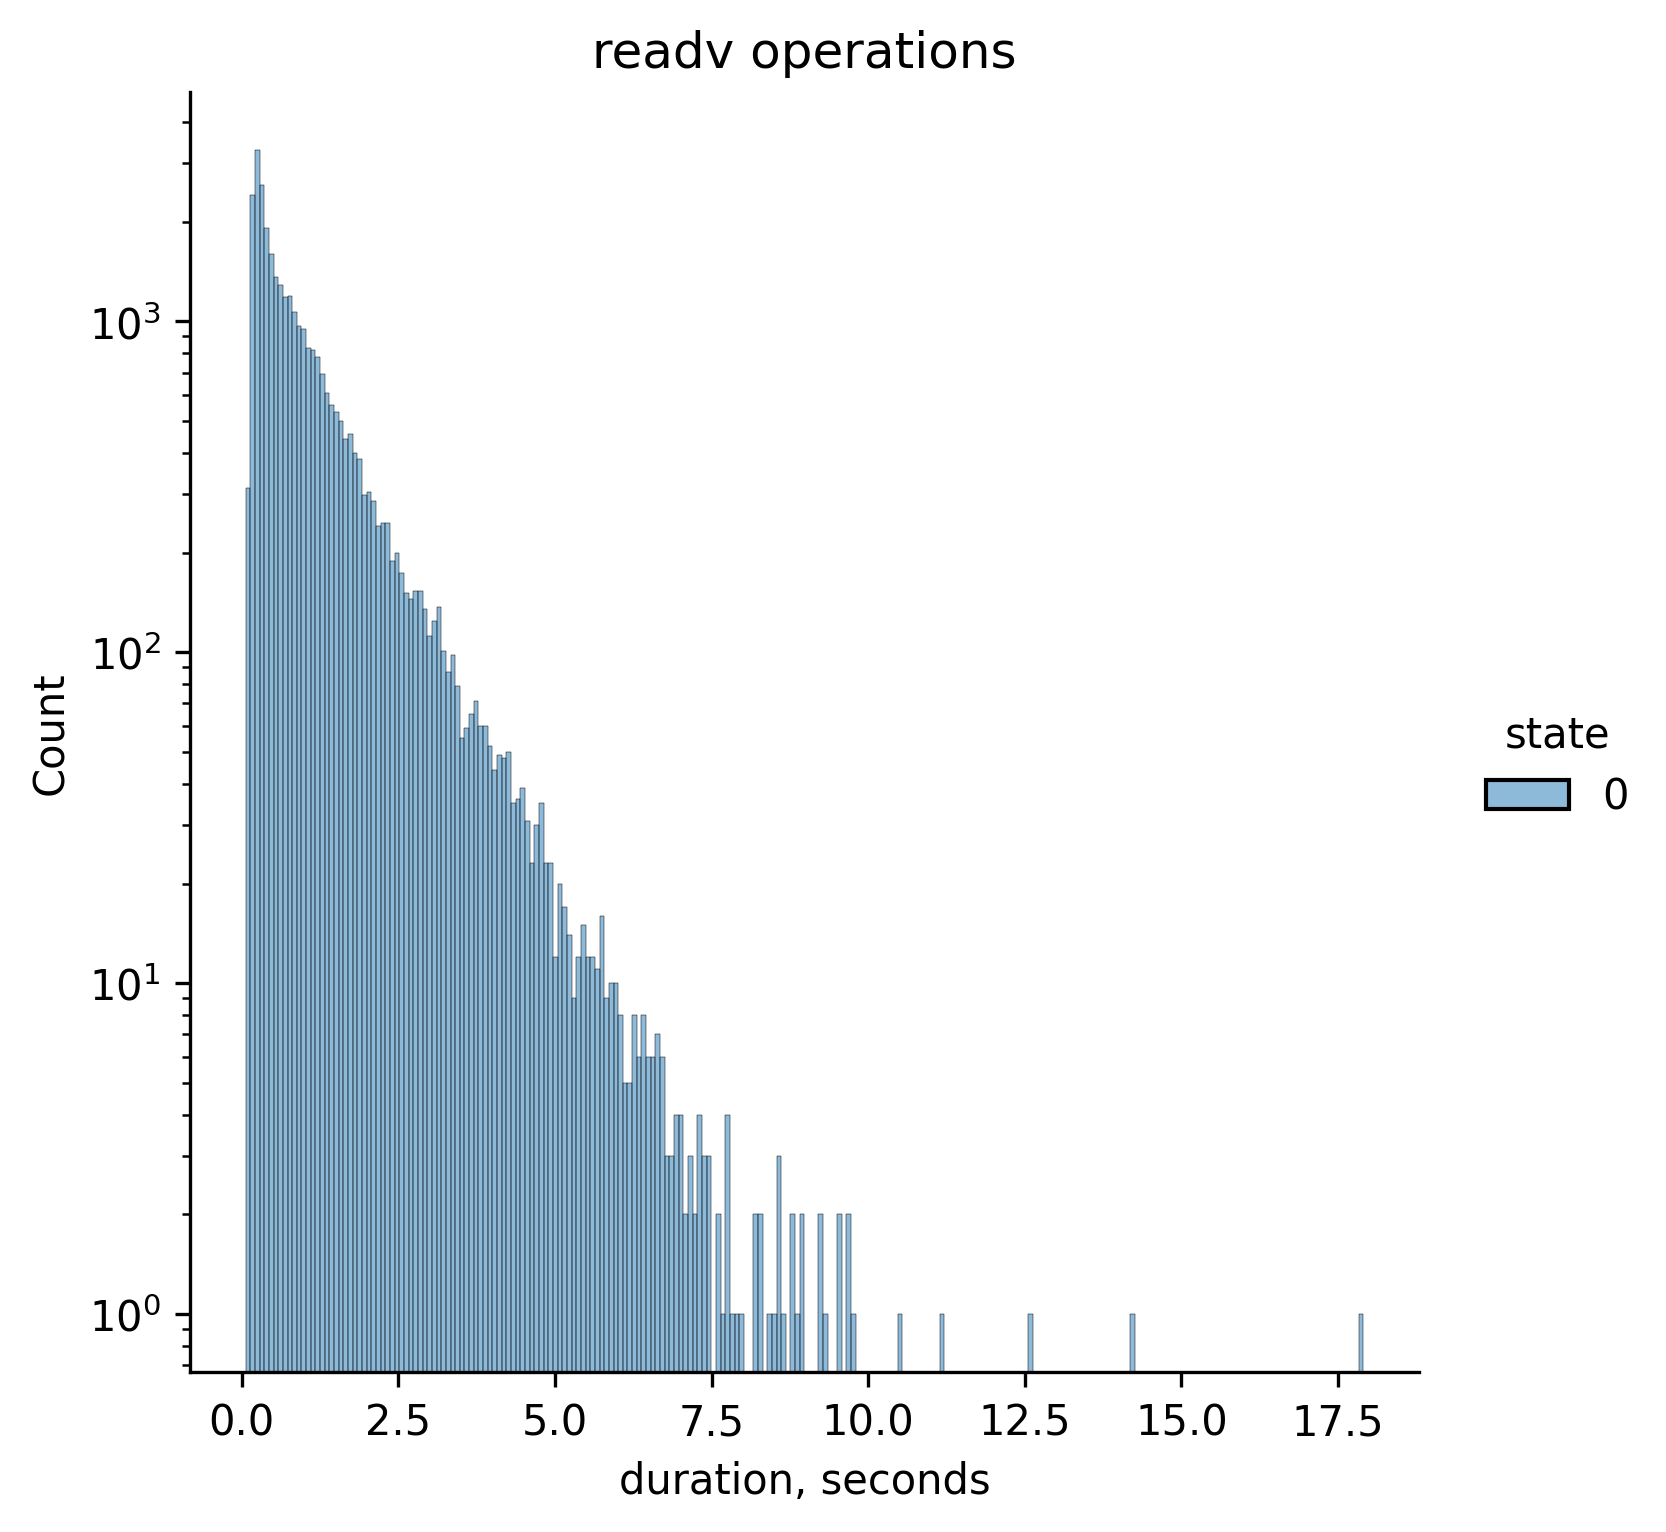
\includegraphics[width=0.45\textwidth,clip]{figures/readv_patched.png}
     \caption{Performance of vector read operations on the original~(left) and update~(right) XrdCeph plugin. State 0 and 1 represent successful and failed reads respecitively. The horizontal axis represents the duration of each operation, noting the difference in scale between the two plots.}
     \label{fig:readv}       % Give a unique label
\end{figure}


\section{Improving metadata operations for checksum requests\label{sec:checksums}}
A request for a checksum (typically using the adler32 algorithm) can proceed in one of two ways (assuming a valid file, etc.). Firstly, if no checksum has previously been computed. Here, the file is read back to the XRootD gateway and the checksum computed. This computed checksum is stored in ceph as metadata on the first object of the file, and the resulting checksum returned to the client. The speed of this is calculated as a rate of O($10$)~s/GiB. Secondly, if there is a checksum already computed. In this case the checksum is retried from the object metadata and returned to the client. 

In XRootD, this is technically achieved via a call to an external python program, which connects to Ceph via the rados client python bindings, performs the necessary operations and then disconnects from the cluster. While this is acceptable for cases where the checksum needs to be computed from the file, the setup and teardown of the connection to the cluster can introduce a significant overhead, when the checksum need only be retreived from the metadata. 
To improve this, client-server model is under development. A service runs on each gateway host that already holds the connection to the ceph cluster, the client - the external application called by XRootD - merely connects to the local server and request the checksum for the given file. 

In Fig.~\ref{fig:checksumming} a comparison between the current and development implementation is shown, for the case of checksum retrieval from metatadata only. 
Other development options for checksumming are also being considered, such as implementing checksuming with the XRootD plugin framework, or, to implement on-the-fly checksumming via the HTTP plugins of XRootD, which would avoid the necessity to re-read the data post initial write. 
%
\begin{figure}[h]
     \centering
     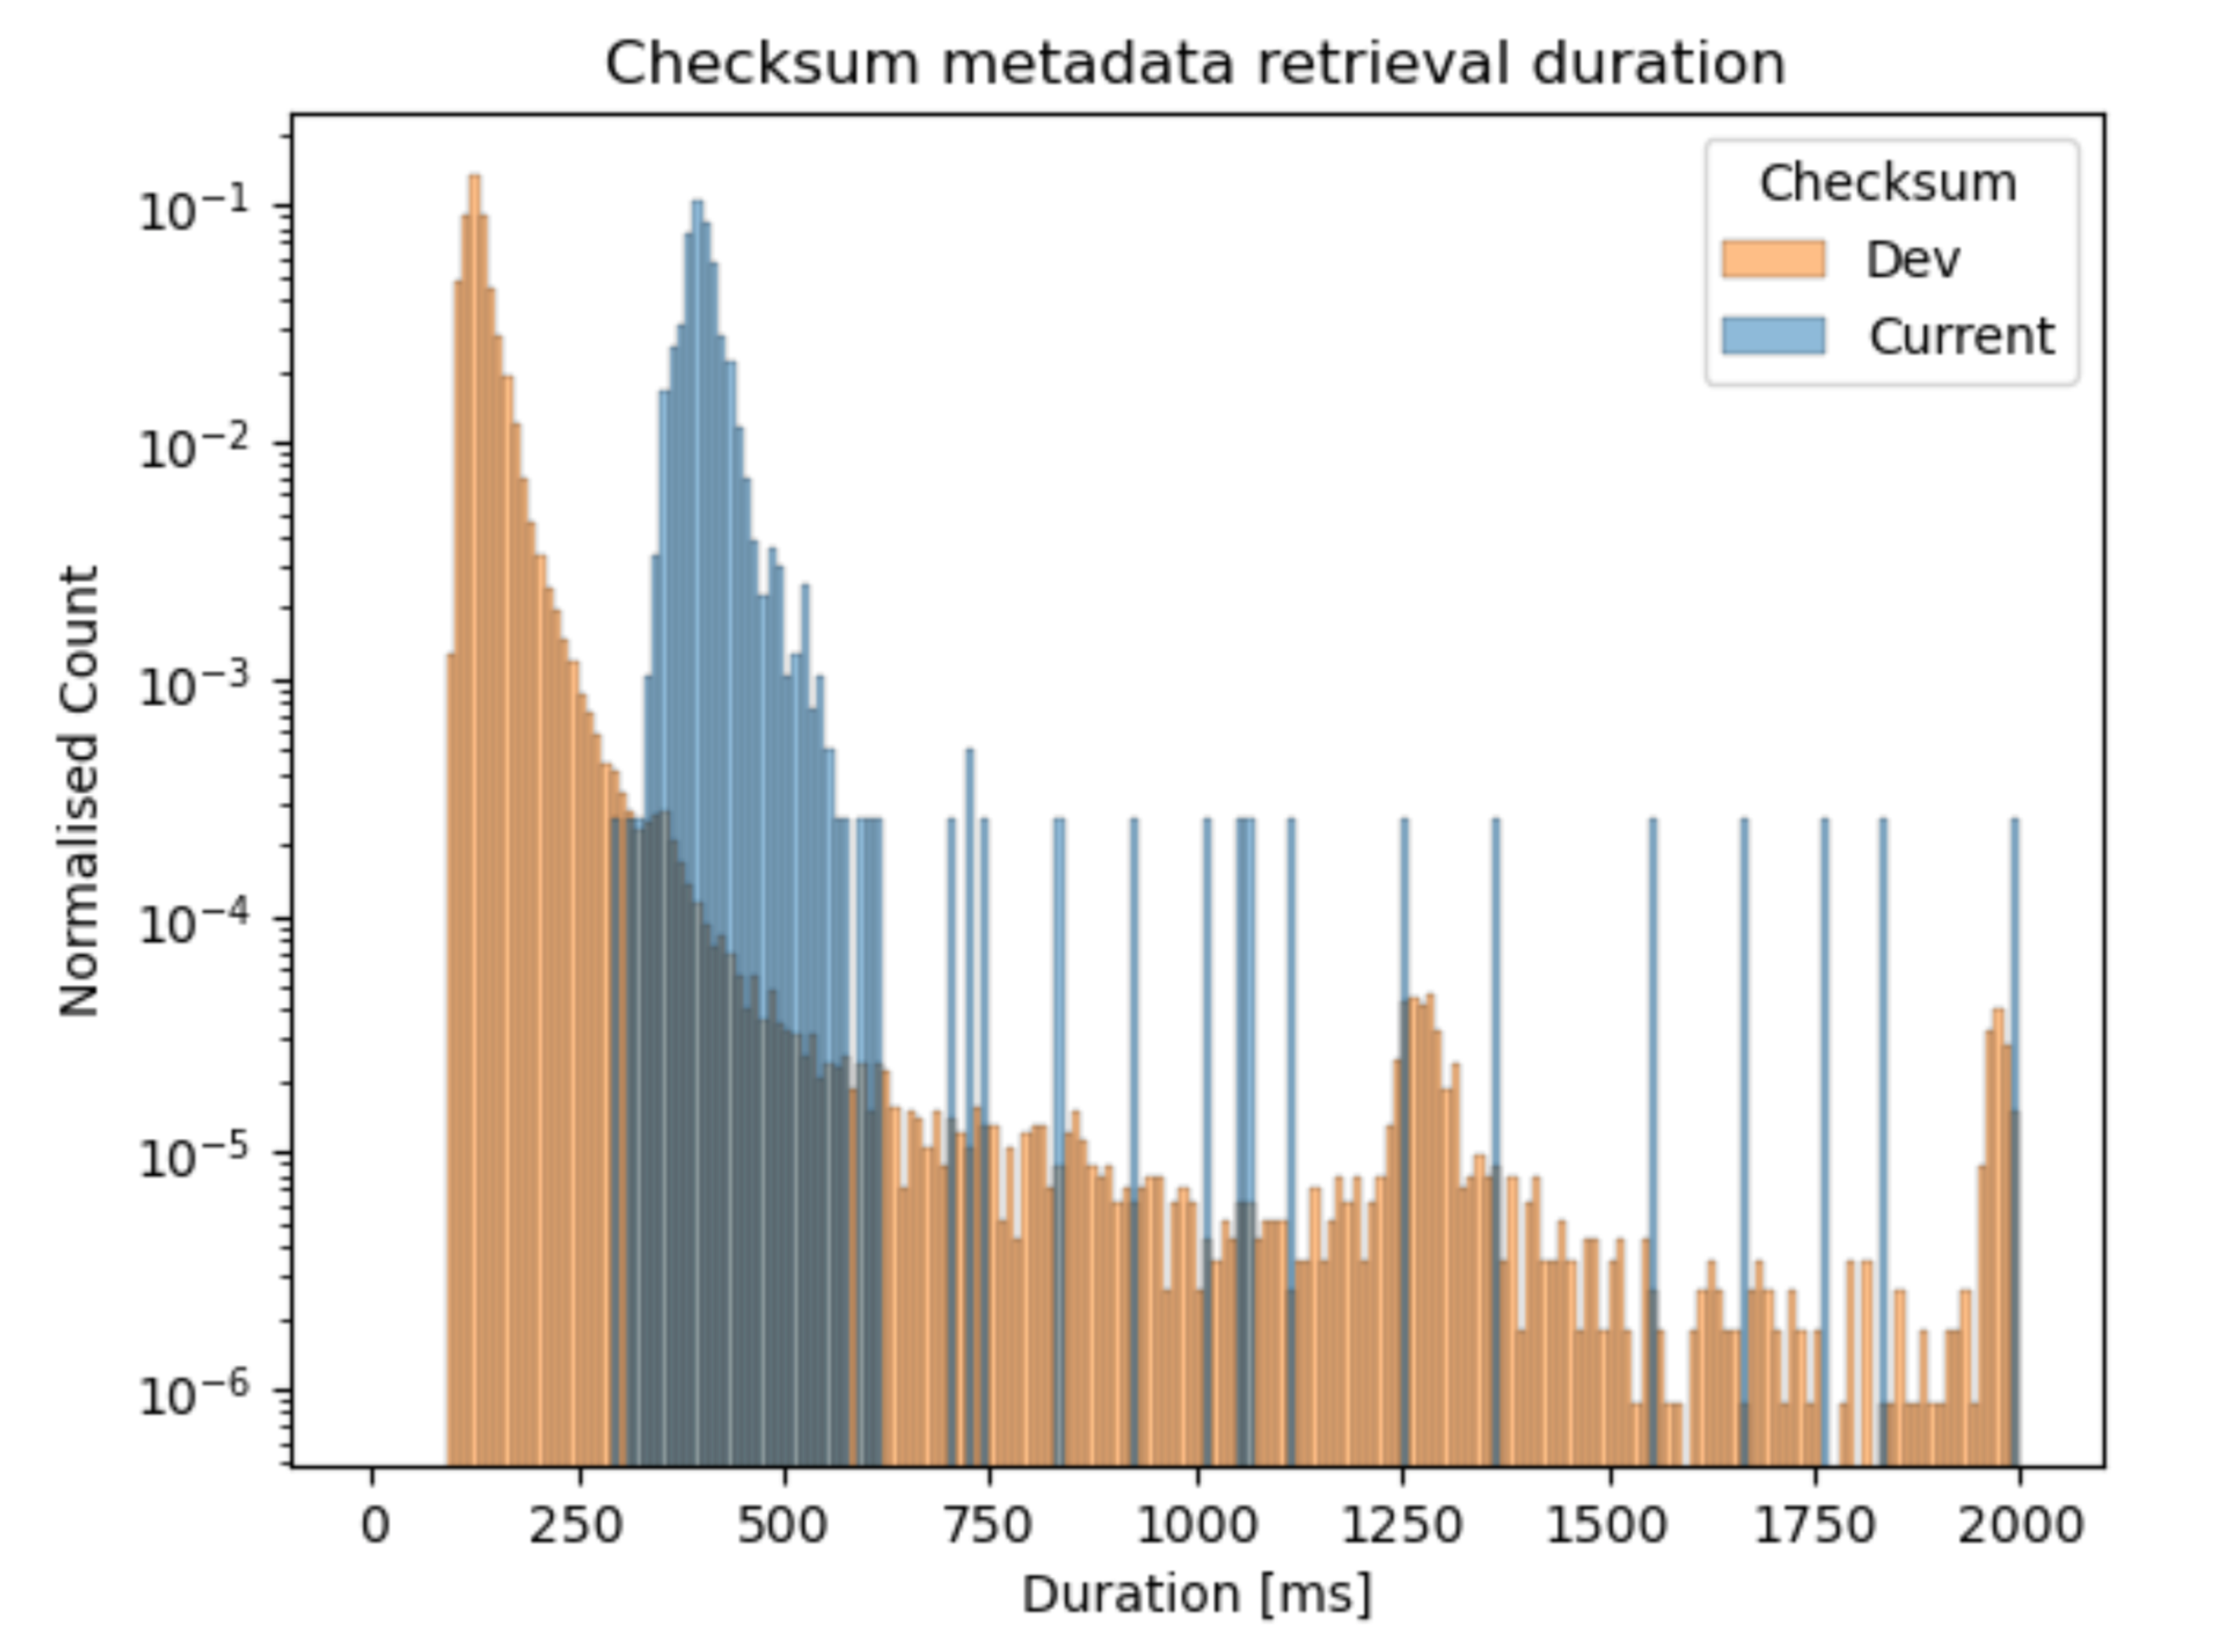
\includegraphics[width=0.45\textwidth,clip]{figures/fig_checksum_meta.pdf}\hfil
     \caption{Comparison of checksum metadata retrieval times using the current implementation and the development client-server approach. Mean retrieval time is observed to improve from $450$~ms to $150$~ms.}
     \label{fig:checksumming}       % Give a unique label
\end{figure}


\section{Resiliance and failover\label{sec:cmsd}}
A DNS round-robin was implemented (at the time of the conference) to distribute the load across the XRootD servers (aka. Gateways) that act as the frontend to the ECHO cluster. While this is a simple and effective solution, it does not accommodate for failure of an individual hosts, or any active load balancing. An alternative approach is to use the CMSD service provide by the XRootD software to actively manage the redirection between a frontend manager and the server hosts. 
%
Figure~\ref{fig:cmsd} illustrates the current configuration that is expected to be deployed into production shortly. A DNS round-robin entry point to two virtual floating IPs. Using keepalived on two XRootD manager hosts to provide failover support in case one of the managers fails. Using the managers and CMSD, the client is redirected to an appropriate server to handle the actual transfer.  
\begin{figure}[h]
     \centering
     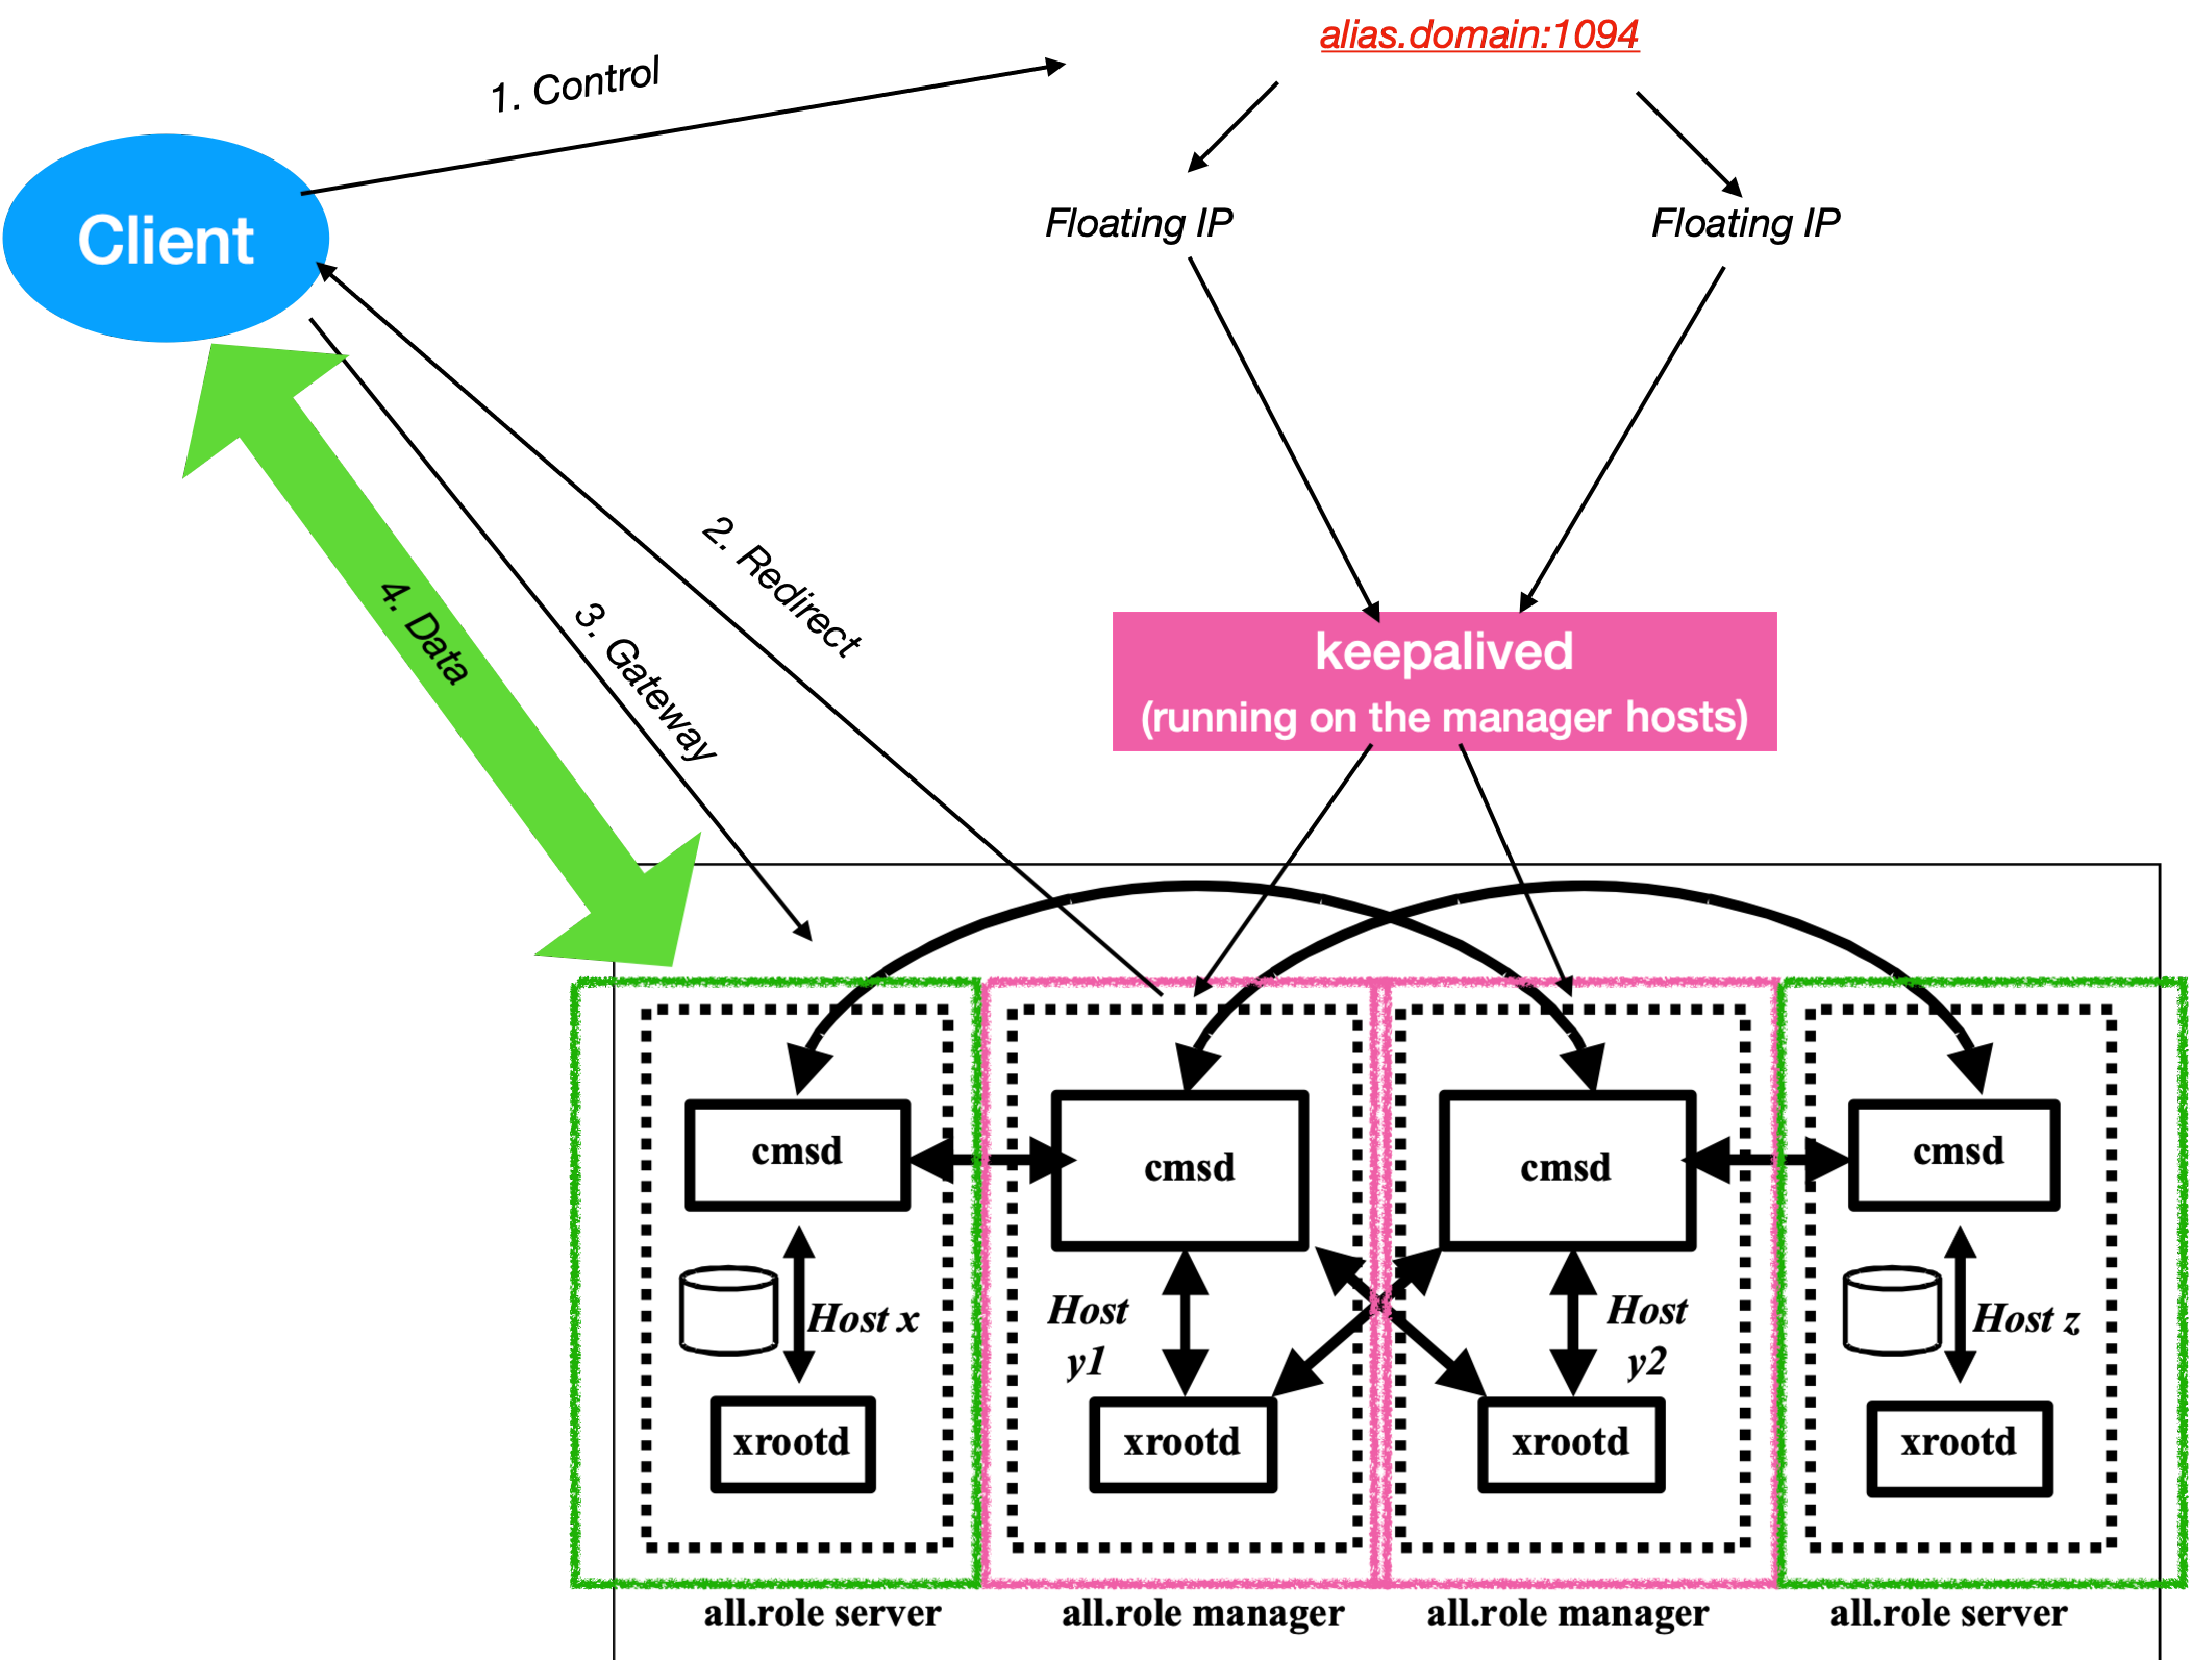
\includegraphics[width=0.75\textwidth,clip]{figures/cmsd.pdf}\hfil
     \caption{Illustration of clustered CMSD configuration using keepalived to provide manager failover. Adapted from Ref.~\cite{xrdcmsd}. Although the figure shows two servers, in practice over 10 servers are connected to the managers.}
     \label{fig:cmsd}       % Give a unique label
\end{figure}

By transitioning from a DNS round-robin to actively managed CMSD setup it is hoped that better resiliance against a problematic cluster will be established, and that active loadbalancing will allow for an even distribution of throughput. Tuning and experience within the production environment will be needed to demonstrate these assertions. 



\section{Summary\label{summary}}
In summary, the ECHO cluster, based at RAL, comprising of XRootD and Ceph,  plays a pivotal role in supporting the data needs of the WLCG and other data-intensive organisations, enabling efficient data distribution, archival, and ensuring data reliability. The combination of XRootD and Ceph technologies provides a versatile and scalable solution that aligns with the demanding requirements of high-energy physics experiments currently at the LHC, and to scale to HL-LHC requirements. 
While scaling of the storage volume itself, and the horizontal scaling of the number of XRootD servers (acting as gateways) is necessary, it is demonstrated that improvements to the architecture and internal software are also necessary to provide efficient, reliable, and cost effective solutions. 
The improvements shown here for read, write and metadata operations, together with improved failover and loadbalancing support, are largely already in place for production opperations, and are demonstrating improved resiliance. 
ECHO already supports LHC and other experiments, and will continue to grow to ensure their future demands. 


% \section{Introduction}
% \label{intro}
% Your text comes here. Separate text sections with
% \section{Section title}
% \label{sec-1}
% For bibliography use \cite{RefJ}
% \subsection{Subsection title}
% \label{sec-2}
% Don't forget to give each section, subsection, subsubsection, and
% paragraph a unique label (see Sect.~\ref{sec-1}).

% For one-column wide figures use syntax of figure~\ref{fig-1}
% \begin{figure}[h]
% % Use the relevant command for your figure-insertion program
% % to insert the figure file.
% \centering
% \includegraphics[width=1cm,clip]{tiger}
% \caption{Please write your figure caption here}
% \label{fig-1}       % Give a unique label
% \end{figure}

% For two-column wide figures use syntax of figure~\ref{fig-2}
% \begin{figure*}
% \centering
% % Use the relevant command for your figure-insertion program
% % to insert the figure file. See example above.
% % If not, use
% \vspace*{5cm}       % Give the correct figure height in cm
% \caption{Please write your figure caption here}
% \label{fig-2}       % Give a unique label
% \end{figure*}

% For figure with sidecaption legend use syntax of figure
% \begin{figure}
% % Use the relevant command for your figure-insertion program
% % to insert the figure file.
% \centering
% \sidecaption
% \includegraphics[width=5cm,clip]{tiger}
% \caption{Please write your figure caption here}
% \label{fig-3}       % Give a unique label
% \end{figure}

% For tables use syntax in table~\ref{tab-1}.
% \begin{table}
% \centering
% \caption{Please write your table caption here}
% \label{tab-1}       % Give a unique label
% % For LaTeX tables you can use
% \begin{tabular}{lll}
% \hline
% first & second & third  \\\hline
% number & number & number \\
% number & number & number \\\hline
% \end{tabular}
% % Or use
% \vspace*{5cm}  % with the correct table height
% \end{table}
% %

\bibliography{echo}

% BibTeX or Biber users please use (the style is already called in the class, ensure that the "woc.bst" style is in your local directory)
% \bibliography{name or your bibliography database}
%
% % Non-BibTeX users please use
% %
% \begin{thebibliography}{}
% %
% % and use \bibitem to create references.
% %
% \bibitem{RefJ}
% % Format for Journal Reference
% Journal Author, Journal \textbf{Volume}, page numbers (year)
% % Format for books
% \bibitem{RefB}
% Book Author, \textit{Book title} (Publisher, place, year) page numbers
% % etc
% \end{thebibliography}

\end{document}

% end of file template.tex
